\documentclass{beamer}
\usetheme{Antibes}
\usecolortheme{beaver}
% \setbeamertemplate{note page}[plain]
% \setbeameroption{show notes on second screen}
\usepackage{fontspec} % Set font families
\setmonofont{UbuntuMono Nerd Font Mono}
\graphicspath{{../img}} % Path to images
\usepackage{graphicx}
\usepackage{xcolor} % Colours
\usepackage{caption} % caption floats
\usepackage{tabularx}
\usepackage{float}
\usepackage[newfloat,outputdir=build]{minted} % source code blocks
\definecolor{codebg}{rgb}{0.9, 0.9, 0.9}
\usepackage{algorithm}
\usepackage{algpseudocode}
\usepackage{mathtools}
\usepackage{amsfonts}

% \newenvironment{code}{\captionsetup{type=listing}}{}
% \SetupFloatingEnvironment{listing}{name=Listing}
% \newcommand\Smallfont{\fontsize{10}{7.2}\selectfont}

\usepackage[backend=biber]{biblatex}
\addbibresource{/home/ramprakash/Documents/notes/bib/datacompr.bib}
\addbibresource{/home/ramprakash/Documents/notes/bib/wavelets.bib}

\usepackage{csquotes}

\logo{
\includegraphics[height=0.6cm]{New_NIE_Logo.png}}

\title{A Study \& Implementation of the Embedded Zerotree Wavelet Algorithm}
\author{
    C. Ramprakash (4NI18EC019) \\ Skanda Prasad (4NI18EC085)
}
\institute[NIE]{
    Under the guidance of Dr. Raghu J. Mandya \& Dr. Narasimha Kaulgud \\
    Department of ECE
    \\
    The National Institute of Engineering, Mysuru
}
\date{August 2021}

\begin{document}

\maketitle

\begin{frame}{Outline}
    \tableofcontents
\end{frame}


\section{Background}
\begin{frame}{Data compression}
    \begin{figure}[H]
        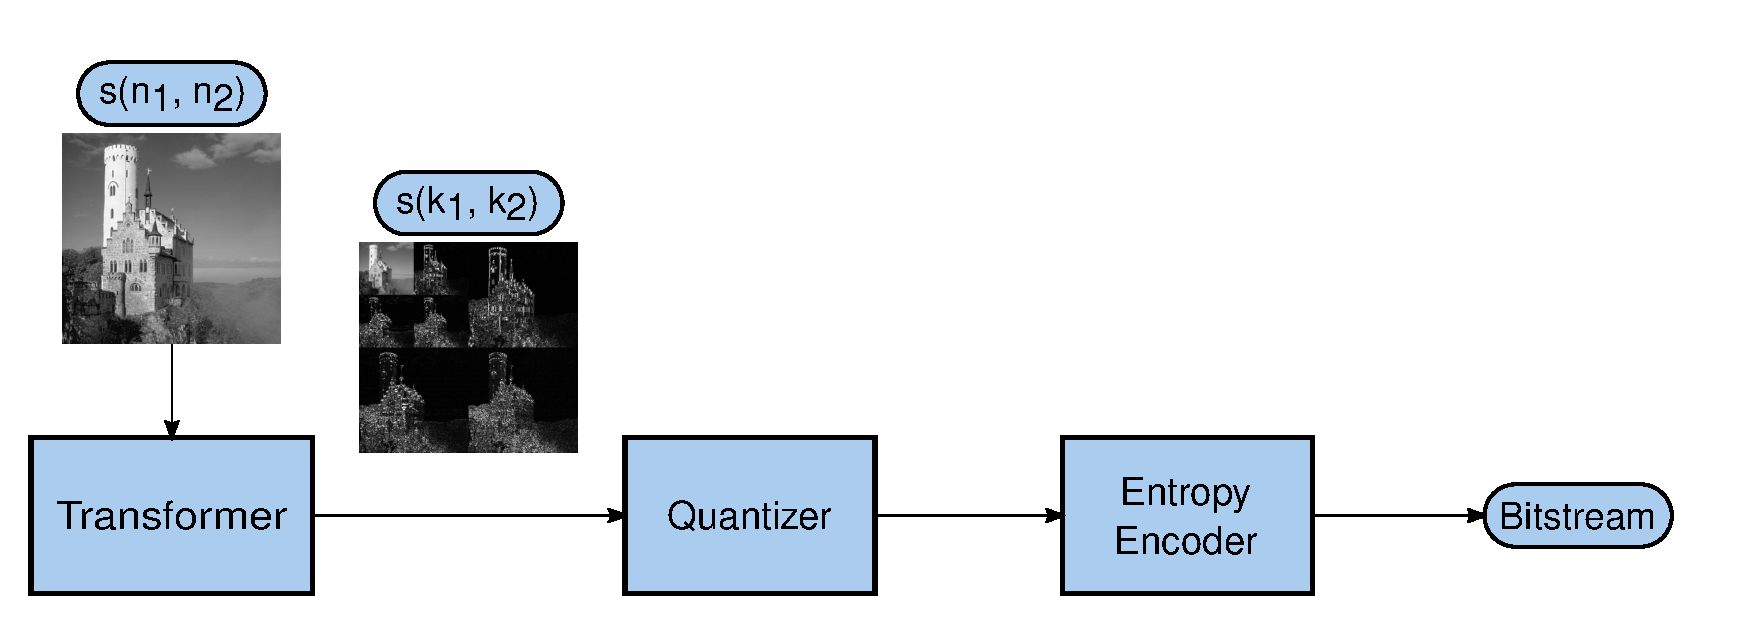
\includegraphics[scale=0.4]{block-diag_shrunk.pdf}
        \caption{Transform coder: Generalised \cite{shap1993}}
    \end{figure}
\end{frame}

\begin{frame}{Data compression}
    A few notable transforms include:
    \begin{itemize}
        \item Discrete Fourier Transform (DFT)
        \item Discrete Cosine Transform (DCT)
        \item Discrete Wavelet Transform (DWT)
    \end{itemize}
\end{frame}

\begin{frame}{Why choose the DWT over others?}
    \begin{itemize}
        \item The ability to truncate (stop) the encoding of bits, without
            significant loss of information
        \item DWT is more resilient to artefact formation (e.g. box artefacts)
    \end{itemize}
\end{frame}

\begin{frame}{The embedded zerotree wavelet algorithm}
    The algorithm is anchored on these key concepts: \cite{shap1993, sayood_datac}
    \vspace{0.5cm}

    \begin{enumerate}
        \item Decompose image into hierarchical sub-bands (using DWT)
        \item Exploit the fact that a single coefficient in a smaller sub-band
            may represent the same spatial location as multiple coefficients in
            \textit{other sub-bands}
        \item Successive-approximation quantization
        \item Compression using an entropy coding technique that is lossless
            such as adaptive arithmetic coding
    \end{enumerate}
\end{frame}

\begin{frame}{Limitations}
    \begin{itemize}
        \item Assumes that only a particular sub-band (\textit{LL}) is split iteratively
        \item Incapable of exploiting spatial redundancies present in
            coefficients \textit{within the same sub-band}
    \end{itemize}
\end{frame}

\section{Problem statement}
\begin{frame}{Problem statement}
    To implement the \textit{Embedded Zerotree Wavelet} algorithm for image
    compression as a C library, and study its performance under various
    circumstances.
\end{frame}

\section{Implementation}
\begin{frame}{Design Constraints}
    \begin{itemize}
        \item The images are assumed to be square in shape
        \item The dimensions of the image are assumed to be exact powers of two
        \item The images are in greyscale
        \item The entropy encoder has been left out of our implementation for simplicity
    \end{itemize}
\end{frame}
\begin{frame}{Software implementation: Wavelet transform}
    \begin{itemize}
        \item External library for computing DWT \cite{rpwavelib}
        \item We have developed a quad-tree data-structure for ease of access
            of coefficients at a particular level and sub-band.
        \item We have also developed a hierarchical tree structure that
            represents the significance-map.
    \end{itemize}
\end{frame}

\begin{frame}[fragile]{Software implementation: Sub-band tree}
    \begin{columns}
        \begin{column}{0.5\textwidth}
            \begin{minted}[bgcolor=codebg, fontsize=\scriptsize]{c}
enum sb_type {
    LL,
    HL,
    LH,
    HH,
    ROOT
};
typedef struct SBtree_node {
    struct SBtree_node *ll;
    struct SBtree_node *hl;
    struct SBtree_node *lh;
    struct SBtree_node *hh;
    double *coeffs;
    enum sb_type type;
} SBtree_node;
            \end{minted}
        \end{column}
        \begin{column}{0.5\textwidth}
            \begin{figure}[H]
                \centering
                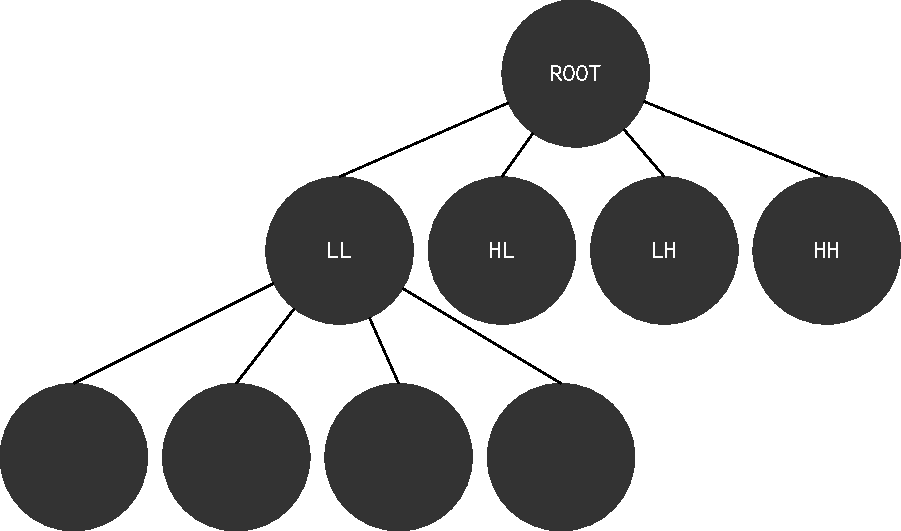
\includegraphics[scale=0.35]{sbtree.pdf}
                \caption{Hierarchical sub-band tree}
            \end{figure}
        \end{column}
    \end{columns}
\end{frame}

\begin{frame}[fragile]{Software implementation: Significance-map tree}
    \begin{columns}
        \begin{column}{0.6\textwidth}
            \begin{minted}[bgcolor=codebg, fontsize=\scriptsize]{c}
enum smap_symbol { // significance map value
    SP = 0, // Significant Positive
    SN = 1, // Significant Negative
    IZ = 2, // Isolated Zero
    ZR = 3, // Zerotree Root
    U = -1 // Unitialized
};
typedef struct Smap_tree_node {
    double coeff;
    struct Smap_tree_node *parent;
    struct Smap_tree_node *children[4];
    char isroot : 1;
    enum smap_symbol type;
    unsigned char not_available;
} Smap_tree_node;
            \end{minted}
        \end{column}
        \begin{column}{0.4\textwidth}
            \begin{figure}[H]
                \centering
                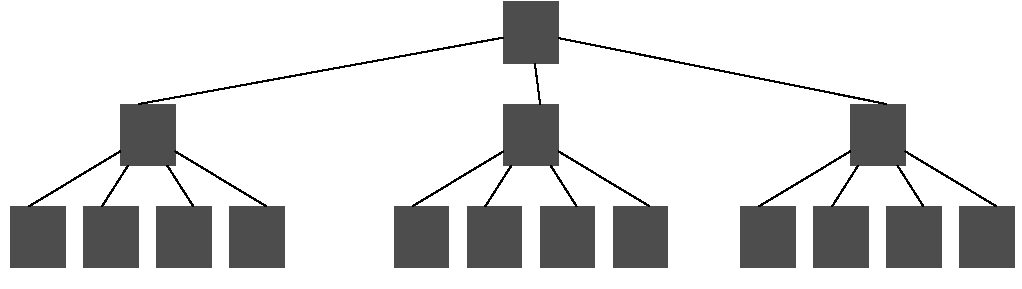
\includegraphics[scale=0.25]{smap.pdf}
                \caption{Significance-map tree}
            \end{figure}
        \end{column}
    \end{columns}
\end{frame}

\begin{frame}{The dominant pass}
    \begin{columns}
        \begin{column}{0.8\textwidth}
            \begin{algorithm}[H]
                \caption{Dominant pass}
                \label{alg:dompass}
                \scriptsize
                \begin{algorithmic}
                    \Require $smap\_tree\_root$ \Comment{Root of a significance map tree}
                    \Require $threshold \in \mathbb{Z}^+$
                    \State $node \gets \text{NULL}$
                    % \State $threshold \gets 2^{\lfloor\log_2{MAX(coefficients)}\rfloor}$\\
                    \ForAll{$node \in \text{level order of } smap\_tree\_root$}
                        \State $check\_descendants(node, threshold)$
                        \If{node is SP or SN or IZ}
                            \State $dominant\_list \gets (dominant\_list, current\_node)$
                        \ElsIf{node is ZR}
                            \If{parent of node is not ZR or node is the root}
                                \State $dominant\_list \gets (dominant\_list, current\_node)$
                            \EndIf
                        \EndIf
                    \EndFor
                \end{algorithmic}
            \end{algorithm}
        \end{column}
        \begin{column}{0.2\textwidth}
            \begin{table}[H]
                \centering
                \scriptsize
                \begin{tabular}{|c|c|}
                    \hline
                    \textbf{Symbol} & \textbf{Binary}\\
                    \hline
                    SP & $00$\\
                    SN & $01$\\
                    IZ & $10$\\
                    ZR & $11$\\
                    \hline
                \end{tabular}
            \end{table}
        \end{column}
    \end{columns}
\end{frame}

\begin{frame}{The subordinate pass}
    \begin{columns}
        \begin{column}{0.7\textwidth}
            \begin{algorithm}[H]
                \caption{EZW}
                \label{alg:subpass}
                \scriptsize
                \begin{algorithmic}
                    \Require $dominant\_list$
                    \Require $threshold \in \mathbb{Z}^+$
                    \State $subordinate\_list \gets \text{NULL}$
                    \State $node \gets \text{NULL}$
                    \ForAll{$node \in dominant\_list$}
                        \State coeff $\gets$ coefficient of node
                        \If{node is SP or SN}
                            \If{$\lvert \text{coeff} \rvert > 1.5 \cdot t$}
                                \State Append a $1$ to $subordinate\_list$
                            \Else
                                \State Append a $0$ to $subordinate\_list$
                            \EndIf
                        \Else
                            \State Append a $0$ to $subordinate\_list$
                        \EndIf
                    \EndFor
                \end{algorithmic}
            \end{algorithm}
        \end{column}
    \end{columns}
\end{frame}

\begin{frame}{The compression algorithm}
    \begin{columns}
        \begin{column}{0.9\textwidth}
            \begin{algorithm}[H]
                \caption{EZW Compression}
                \label{alg:ezwcomp}
                \scriptsize
                \begin{algorithmic}
                    \Require $smap\_tree\_root$ \Comment{Root of a significance map tree}
                    \Require $min\_threshold \ge 0$
                    \State $node \gets \text{NULL}$
                    \State $threshold \gets 2^{\lfloor\log_2{MAX(\text{coefficients of } smap\_tree\_root)}\rfloor}$
                    \While{$threshold > min\_threshold$}
                        \State $dominant\_list \gets$ dominant\_pass(smap\_tree\_root, threshold)
                        \State $subordinate\_list \gets subordinate\_pass(dominant\_list, threshold)$
                        \State Write data to file
                        \State $threshold \gets threshold/2$
                    \EndWhile
                \end{algorithmic}
            \end{algorithm}
        \end{column}
    \end{columns}
\end{frame}

\begin{frame}{The decompression algorithm}
    \begin{columns}
        \begin{column}{\textwidth}
            \begin{algorithm}[H]
                \caption{EZW Decompression}
                \label{alg:ezwdecomp}
                \scriptsize
                \begin{algorithmic}
                    \Require $compressed\_file$
                    \State $dominant\_list \gets \text{NULL}$
                    \State $subordinate\_list \gets \text{NULL}$
                    \ForAll{$dominant\_list, subordinate\_list$}
                        \State Approximate coefficients in $dominant\_list$
                        \State Refine respective coefficients using $subordinate\_list$
                        \State Write data to file
                    \EndFor
                \end{algorithmic}
            \end{algorithm}
        \end{column}
    \end{columns}
\end{frame}

\section{Conclusion}
\subsection{Results}
\begin{frame}
    \begin{table}[H]
    \scriptsize
    \begin{tabular}{|c|c|c|c|}
        \hline
        \textbf{Image} & \textbf{Original size (bytes)} & \textbf{Size after
        compression (bytes)} & \textbf{Iterations}\\
        \hline
        eggs8 & 64 & 46 & 4\\
        eggs8 & 64 & 70 & 5\\
        eggs8 & 64 & 216 & Max\\
        \hline
        eggs16 & 256 & 153 & 6\\
        eggs16 & 256 & 257 & 7\\
        eggs16 & 256 & 621 & Max\\
        \hline
        lichten & 262144 & 198751 & 14\\
        lichten & 262144 & 269263 & 15\\
        lichten & 262144 & 352671 & Max\\
        \hline
    \end{tabular}
\end{table}

\begin{block}{Note}
    The maximum number of iterations for a given image is given by:
    $$Max = \log_2{T_0}$$
\end{block}
\end{frame}

\subsection{Future work}
\begin{frame}
    \begin{itemize}
        \item Write the de-compressor
        \item Include entropy encoder
        \item A multi-core implementation of the algorithm
        \item An FPGA-based hardware accelerator for the algorithm
    \end{itemize}
\end{frame}

\section{References}
\begin{frame}
    \printbibliography
\end{frame}

\section{End}
\begin{frame}
    \centering
    \huge{Thank You}
    \par
    \huge{Questions?}
\end{frame}

\end{document}

